\documentclass{elsarticle}

\usepackage{amsmath}
\usepackage{graphics}
\usepackage{graphicx}
\usepackage{color}
\usepackage{xspace}
\usepackage{url}
\usepackage[utf8]{inputenc}
\usepackage{booktabs}
\usepackage{caption}
\usepackage{subcaption}

% reviews
\newcommand{\todo}[1]        {\textcolor{red}{[TODO] #1}}
\newcommand{\keoma}[1]       {\textcolor{blue}{[Keoma] #1}}
\newcommand{\remy}[1]        {\textcolor{blue}{[Remy] #1}}
\newcommand{\xavi}[1]        {\textcolor{blue}{[Xavi] #1}}
\newcommand{\thomas}[1]      {\textcolor{blue}{[Thomas] #1}}

 % lorem
\newcommand{\lorem}          {\textcolor{green}{Lorem ipsum dolor sit amet, consectetur adipisicing elit, sed do eiusmod tempor incididunt ut labore et dolore magna aliqua. Ut enim ad minim veniam, quis nostrud exercitation ullamco laboris nisi ut aliquip ex ea commodo consequat. Duis aute irure dolor in reprehenderit in voluptate velit esse cillum dolore eu fugiat nulla pariatur. Excepteur sint occaecat cupidatat non proident, sunt in culpa qui officia deserunt mollit anim id est laborum.}}

% shortcuts
\newcommand{\smip}                {SmartMesh~IP\xspace}
\newcommand{\HRNEIGHBORS}         {{\tt HR\_NEIGHBORS}\xspace}
\newcommand{\HRDISCOVERED}        {{\tt HR\_DISCOVERED}\xspace}
\newcommand{\HRDEVICE}            {{\tt HR\_DEVICE}\xspace}
\newcommand{\pathcreate}          {{\tt path\_create}\xspace}
\newcommand{\pathdelete}          {{\tt path\_delete}\xspace}
\newcommand{\motecreate}          {{\tt mote\_create}\xspace}
\newcommand{\moteId}              {{\tt moteId}\xspace}
\newcommand{\PEACHNUMHRNEIGHBORS} {140,897\xspace}
\newcommand{\PEACHNUMSTATS}       {369,276\xspace}
\newcommand{\EVANUMHRNEIGHBORS}   {144,217\xspace}

\graphicspath{{figures/}}

\begin{document}
	
\begin{frontmatter}
    
\date{}
	
\title{(Not so) Intuitive Results from two Real-World\\Low-Power Wireless Mesh Deployments}

\author[inria]{Keoma~Brun-Laguna}
	\ead{keoma.brun@inria.fr}
\author[inria]{R\'emy~L\'eone}
    \ead{remy.leone@inria.fr}
\author[uoc]{Xavier~Vilajosana}
    \ead{xvilajosana@uoc.edu}
\author[inria]{Thomas~Watteyne}
    \ead{thomas.watteyne@inria.fr}

\address[inria]{Inria, EVA team, Paris, France}
\address[uoc]{Univ. Oberta de Catalunya, Barcelona, Catalonia, Spain}



\begin{abstract}
Two wireless network sensors are deployed.
One in a peach orchard and one in a office building.
The two networks are collecting sensor values and network statistics.
This paper presents an in-depth analysis of the statistics, in order to precisely understand the performance of the network.
Nodes in the network exhibit an expected lifetime between 4 and 16~years, with an end-to-end reliability of 100\%.
We show how -- contrary to popular belief -- wireless links are symmetric.
Thanks to the use of Time Slotted Channel Hopping (TSCH), the network topology is very stable, with $\leq$5 link changes per day in the entire network.
\end{abstract}

\begin{keyword}
    WSN, SmartAgriculture, SmartBuilding
\end{keyword}

\end{frontmatter}

%==============================================================================

%======== front-page figure, do not move
\begin{figure}
    \centering
    \includegraphics[width=0.8\textwidth]{orchard}
    \caption{Areal view of the sensor network deployed in the orchard near Mendoza, Argentina.}
    \label{fig:orchard}
\end{figure}

\section{Introduction}
\label{sec:intro}

% the problem

Peaches do not like frost.
If during the blooming season (September in Argentina), temperature gets below $-$3~C for only a couple of hours, the flowers freeze, and no peaches are produced.
In 2013, 85\% of the peach production in the Mendoza region (western Argentina) was lost because of frost events.
Farmers can lose everything in only a couple of hours.
Yet, if they are warned of a frost event a couple of hours ahead, they can install heaters throughout the orchards, and use big fans to move the hot air around.
Fighting the frost events is not the issue, what is hard is predicting it.

% the PEACH project

The goal of the PEACH project~\cite{watteyne16peach} is to predict frost events.
We install sensors around the orchard that measure air temperature, air relative humidity, soil moisture and soil temperature.
We feed the collected data into a database, and by analyzing the data in real-time using machine learning, we identify patterns in the data and predict frost events.

% the architecture

Because of the heavy machinery that moves inside the orchard, using cables to interconnect the sensors is not an option.
The main challenge is to deploy a system that provides both a high end-to-end reliability and a long lifetime without using cables.
We use \smip, an off-the-shelf low-power wireless mesh solution from Linear Technology.
The sensor devices are battery-powered and equipped with a radio.
They form a multi-hop topology, and collaborate to route the data generated by the devices (called ``motes'') to a gateway.
This gateway is connected to the Internet, and forwards the gathered date to the servers in Paris, France.
Data appears on the web interface of the servers seconds after it was gathered by the sensor network.

% the deployment

The network is deployed in a peach orchard of 204~trees, planted in a 50~m~$\times$~100~m area (shown in Fig.~\ref{fig:map}).
The low-power wireless network is composed of 18~sensor motes\footnote{2 motes malfunctioned and are not present on the map.} uniformly distributed between the peach trees, and 3~relay motes to connect the orchard to the gateway some 300~m away.
Each mote is placed in a water-tight box that is fixed on a 4~m high pole (see Fig.~\ref{fig:orchard}).

\begin{figure}
    \begin{minipage}[b]{0.66\textwidth}
        \centering
        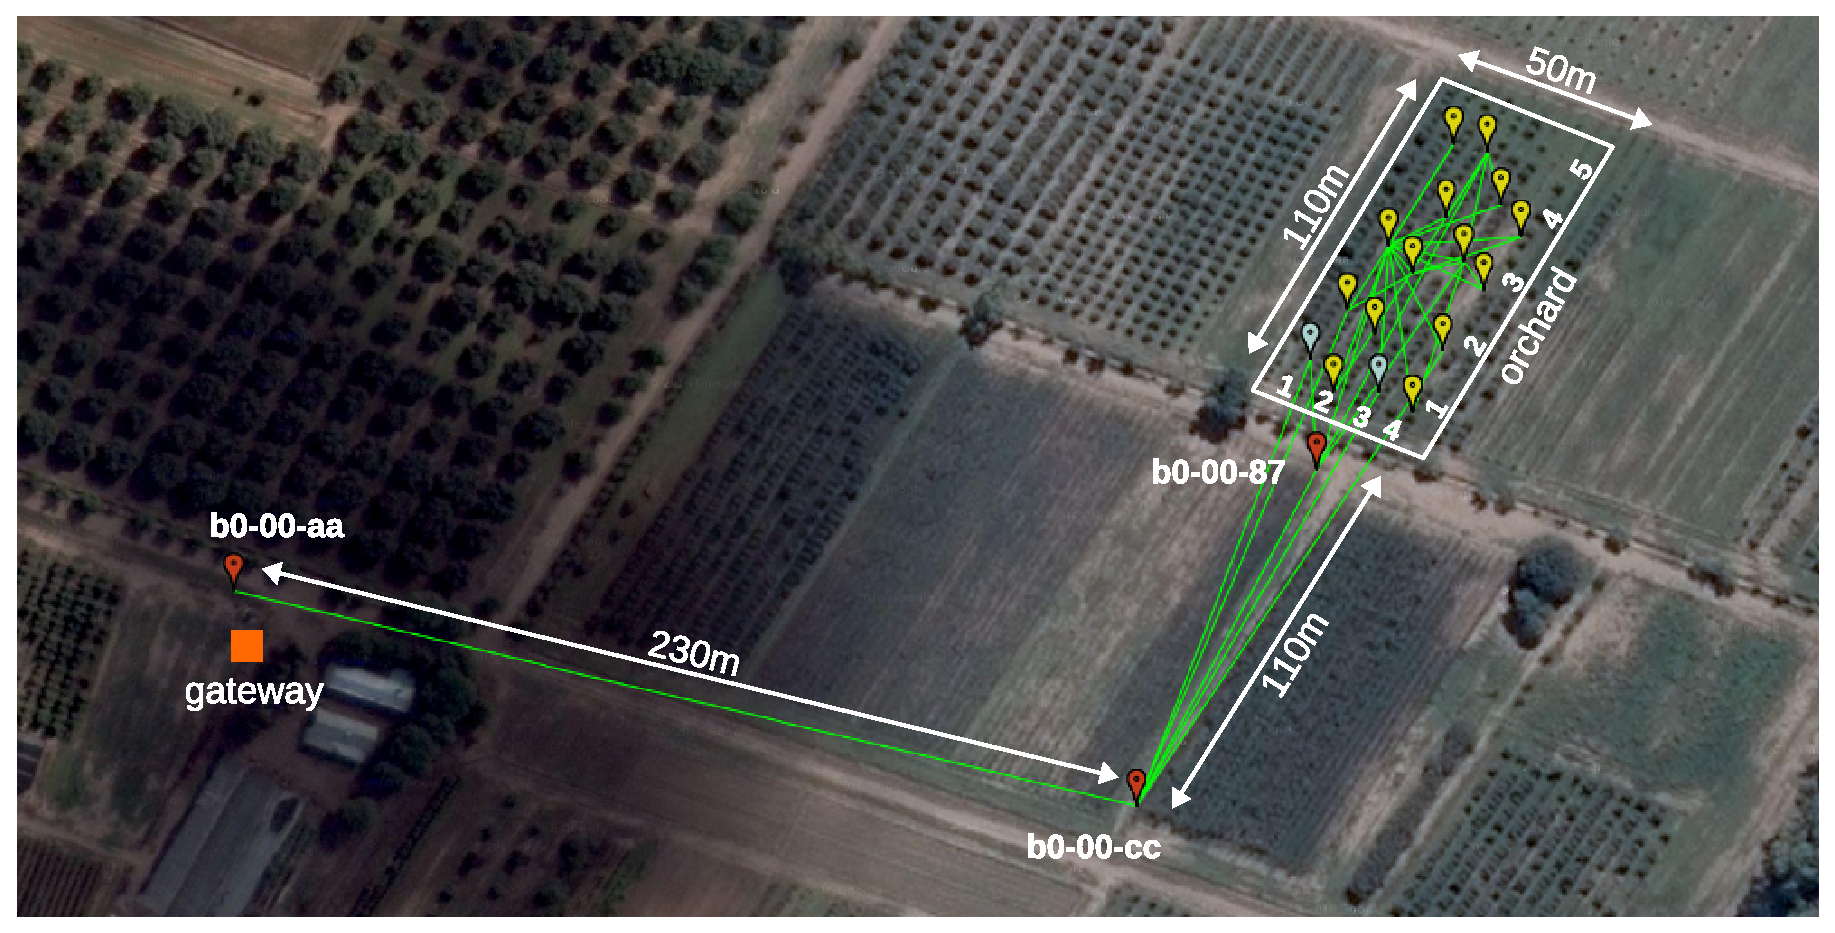
\includegraphics[width=\textwidth]{map_annotated}
        \caption{The wireless motes deployed in the peach orchard in Mendoza, Argentina.\newline}
        \label{fig:map}
    \end{minipage}
    \hfill
    \begin{minipage}[b]{0.3\textwidth}
        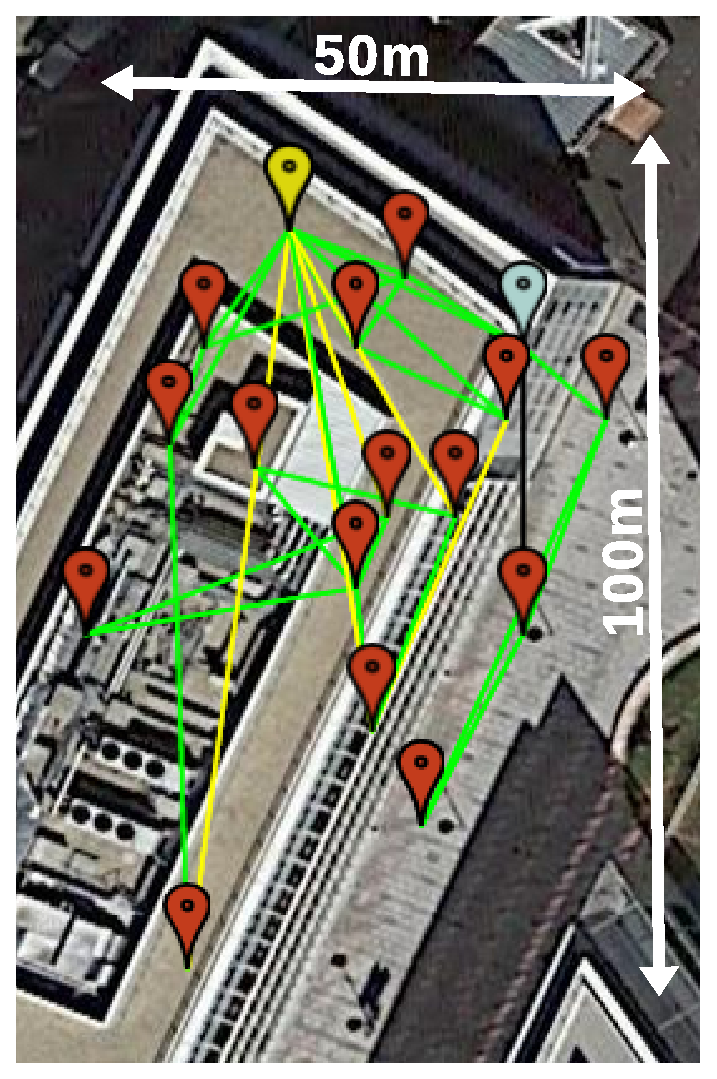
\includegraphics[width=\textwidth]{evalab_map_annotated.eps}
        \caption{The wireless motes deployed in the Inria office building, France.}
    \end{minipage}
\end{figure}

% hardware

In the peach orchard we use four types of \smip devices.
The 2 DC9018 boards feature an external antenna; the 16 DC9003 boards a chip antenna.
These are deployed inside the orchard.
We deploy 3 repeaters outside the orchards to connect the orchard to the gateway.
For the two deployments, the gateway is composed of a Raspberry~Pi single-board computer, and a DC2274 \smip manager.

% technology

The \smip network implements the IEEE802.15.4e standard~\cite{std_ieee802154e_2012}, which includes a channel hopping mechanism to reduce the impact of multipath fading and external interference.
This allows the network to be highly reliable, stable, and extremely low power~\cite{watteyne10mitigating, watteyne09reliability}.

% the data

Each mote produces a temperature value every 30~s, and network statistics every 5~min.
In 3~months of operation, we gathered over 4~million temperature values, and more than 350,000~network statistics.

% the goal of this paper

The goal of this paper is to analyze the network statistics over a 3-month period, and precisely assess the performance of the network.
\\

This paper makes the following contributions:
\begin{itemize}
    \item We confirm that the \smip network exhibits years of battery lifetime and wire-like reliability;
    \item We show that channel hopping causes the network topology to be very stable, with $\leq$5 link changes per day;
    \item Contrary to popular belief, we show that links in the network are symmetric, i.e.~they exhibit the same signal strength in both directions of the same link.
\end{itemize}

% paper organisation

The remainder of this paper is organized as follows.
Section~\ref{sec:collected} describes what statistics we are collecting, and the amount of statistics collected over two periods of 3~months.
Section~\ref{sec:intuitive} presents results that confirm assumptions about what we can expect for real-world \smip deployment.
Section~\ref{sec:notsointuitive} presents not so intuitive results about link symmetry and network stability.
Finally, Section~\ref{sec:conclusion} concludes this paper and discusses further improvements.

%==============================================================================
\section{Statistics Collected}
\label{sec:collected}

% environment

The wireless network is deployed in a peach orchard in Junin, 45~km South-East of Mendoza in Western Argentina.
No other electronic devices are present in the field.
Farmers work inside the field with heavy machinery for 1-2~h every 20~days approximately.
In the region, air temperature ranges between $-$9~C in winter (May-October) to +38~C in summer (November-April).
Because of the sunny weather, day/night temperature swings of 10+~C are not uncommon in winter.

% events and HR

Each device in the network produces both sensor data and network statistics.
Network statistics can be separated in Events and Health Reports messages.
\textit{Event} messages are non-periodic notifications the network sends when a network event happens (e.g.~a node joins/leaves the network, a link is created/deleted).
\textit{Health Report} (HR) messages are sent periodically by each mote; they contain counters and statistics about that mote.
HRs are used to assess the overall health of the network.

% number received and remainder

Table~\ref{tab:msg_stats} summarizes the number of events and HRs gathered during the two periods of 3~month.
In the remainder of this section, we detail the meaning of each of the statistics.

\begin{table}
    \centering
    \begin{tabular}{|l|r|r|}
        \toprule
        \multicolumn{1}{|c|}{type} & \multicolumn{1}{|c|}{PEACH} & \multicolumn{1}{|c|}{EVAlab} \\ \hline
        \hline
        \motecreate     &     133     &   85 \\ \hline
        \pathcreate     &   4,098     &   2,149 \\ \hline
        \pathdelete     &   3,653     &   2,070 \\ \hline
        \HRDEVICE       & 132,758     &   144,270 \\ \hline
        \HRDISCOVERED   &  87,737     &   126,906 \\ \hline
        \HRNEIGHBORS    & \PEACHNUMHRNEIGHBORS & \EVANUMHRNEIGHBORS\\ \hline
    \end{tabular}
    \caption{The number of statistics collected over the 3~month period.}
    \label{tab:msg_stats}
\end{table}

% - - - - - - - - - - - - - -
\textbf{\motecreate.}
Each node in a \smip network can periodically send beacons to announce the presence of the network.
When a mote wants to join a network, it listens for those beacons.
Once it has heard a number of those, it starts a security handshake with the network.
During that handshake, the \smip manager sends a \motecreate event notification over its serial port.
This is the event we log\footnote{Normally, each mote generates a single \motecreate event. Due to power issues at the manager side, the network restarted a couple of times and new events were created.}.
It contains, among other information, the association between the newly-joined device's 8-byte MAC address and its 2-byte \moteId.

% - - - - - - - - - - - - - -
\textbf{\pathcreate and \pathdelete.}
In \smip terminology, a ``path'' is the link-layer resource that allows two neighbor nodes to communicate\footnote{~In more classical networking terminology, this is often referred to as a ``link''. We use the terms ``path'' and ``link'' interchangeably in this paper.}.
Each time a mote starts communicating with a new neighbor (e.g.~its routing parent), a \pathcreate event is produced.
Similarly, each time a mote \textit{stops} communicating with a neighbor (e.g.~it changes routing parent), a \pathdelete event is produced.
We log both messages.

% - - - - - - - - - - - - - -
\textbf{\HRDEVICE.}
Each network device produces a \HRDEVICE every 15~min.
This health report contains counters/statistics internal to the mote, such as its current battery voltage, temperature, or total number of messages sent.

% - - - - - - - - - - - - - -
\textbf{\HRDISCOVERED.}
\smip nodes continuously monitor their surroundings to discover neighbor nodes.
Every 15~min, each node produces an \HRDISCOVERED health report that contains the list of ``discovered'' neighbors, and the associate signal strength it heard them at.
These discovered neighbors can potentially be used in the future as neighbors the node communicates with.

% - - - - - - - - - - - - - -
\textbf{\HRNEIGHBORS.}
Two nodes are neighbors when link-layer resources are installed for them to communicate.
The neighbors of a node are a subset of the discovered neighbors.
Every 15~min, each note generates an \HRNEIGHBORS health report that contains its list of neighbors.
These messages also specifies per-neighbor counters, such as the number of link-layer retransmissions.

% analysis

After 3~months of operation, we have collected \PEACHNUMSTATS~network statistics (see Table~\ref{tab:msg_stats}).
The goal of the next section is to present the main results from analyzing this information.
We group these results in two categories.
``Intuitive'' results (Section~\ref{sec:intuitive}) are results that confirm the performance expected from a \smip network.
``Not so intuitive'' results (Section~\ref{sec:notsointuitive}) are results that we believe go against popular belief.
This classification is necessarily subjective.

Possibly due to power line failure at the network manager side, the network experienced some restarting.
For this reason, some analysis presented in the next sections are done in shorter period.
As a side effect, this allows us to verify the network formation and joining process.

%==============================================================================
\section{Intuitive Results}
\label{sec:intuitive}

Previous publications~\cite{watteyne16peach,watteyne10mitigating,watteyne09reliability,watteyne15industrial} underline the performance of TSCH networks in general, and \smip in particular.
Standardization work in the IETF 6TiSCH working group\footnote{~\url{https://tools.ietf.org/wg/6tisch/charters}} around TSCH networks further illustrates the move of the industry towards this type of networking technology.
So while we expect good performance from the network, this section verifies that this is indeed the case.
We start by looking at two physical-layer metrics: RSSI vs Distance (Section~\ref{sec:rssi_distance}) and PDR vs. RSSI (Section~\ref{sec:waterfall}).
While these have no dependency on TSCH (the type of medium access), they allow us to verify the overall connectivity in the network.
We then look at key performance indicators of \smip networks: end-to-end reliability (Section~\ref{sec:net_reliability}) and network lifetime (Section~\ref{sec:lifetime}).

%------------------------------------------------------------------------------
\subsection{RSSI vs. Distance}
\label{sec:rssi_distance}

The Friis transmission model~\cite{saunders07antennas} gives the relationship between the Received Signal Strength (RSSI)\footnote{~Strictly speaking, the RSSI is the Received Signal Strength \textit{Indicator}, a value returned by radio chip. Because of its prevalence in low-power wireless literature, we use it RSS and RSSI interchangeably.} in free space.
While it does \textit{not} apply directly to our real-world deployment, we note in Fig.~\ref{fig:pister_hack} that the individual RSSI values are located between the Friis model, and the Friis model offset by $-$40~dB.
This corroborates the results from~\cite{zats10wireless}.

\begin{figure}[h]
    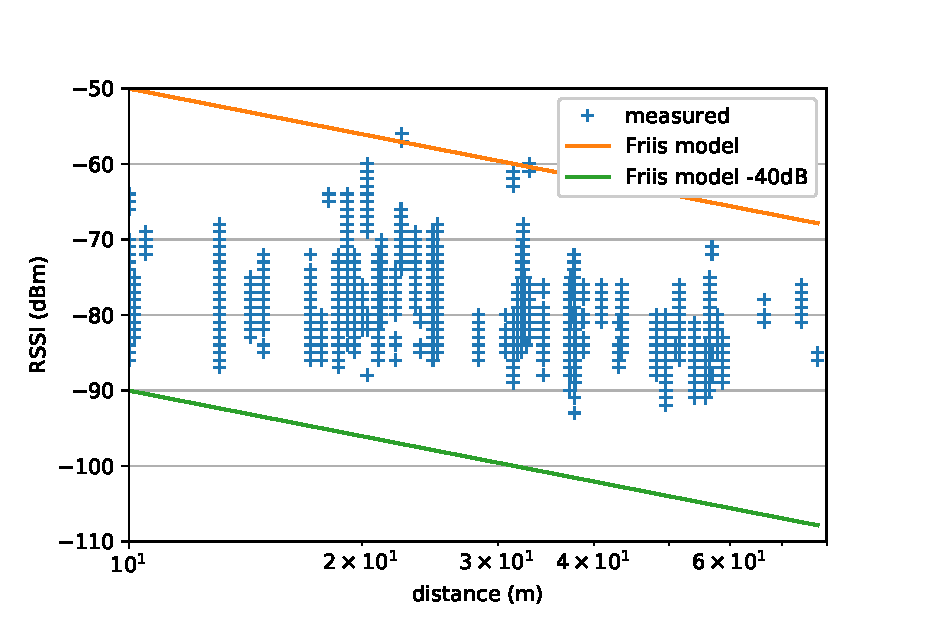
\includegraphics[width=0.5\textwidth]{pister_hack_peach.eps}
    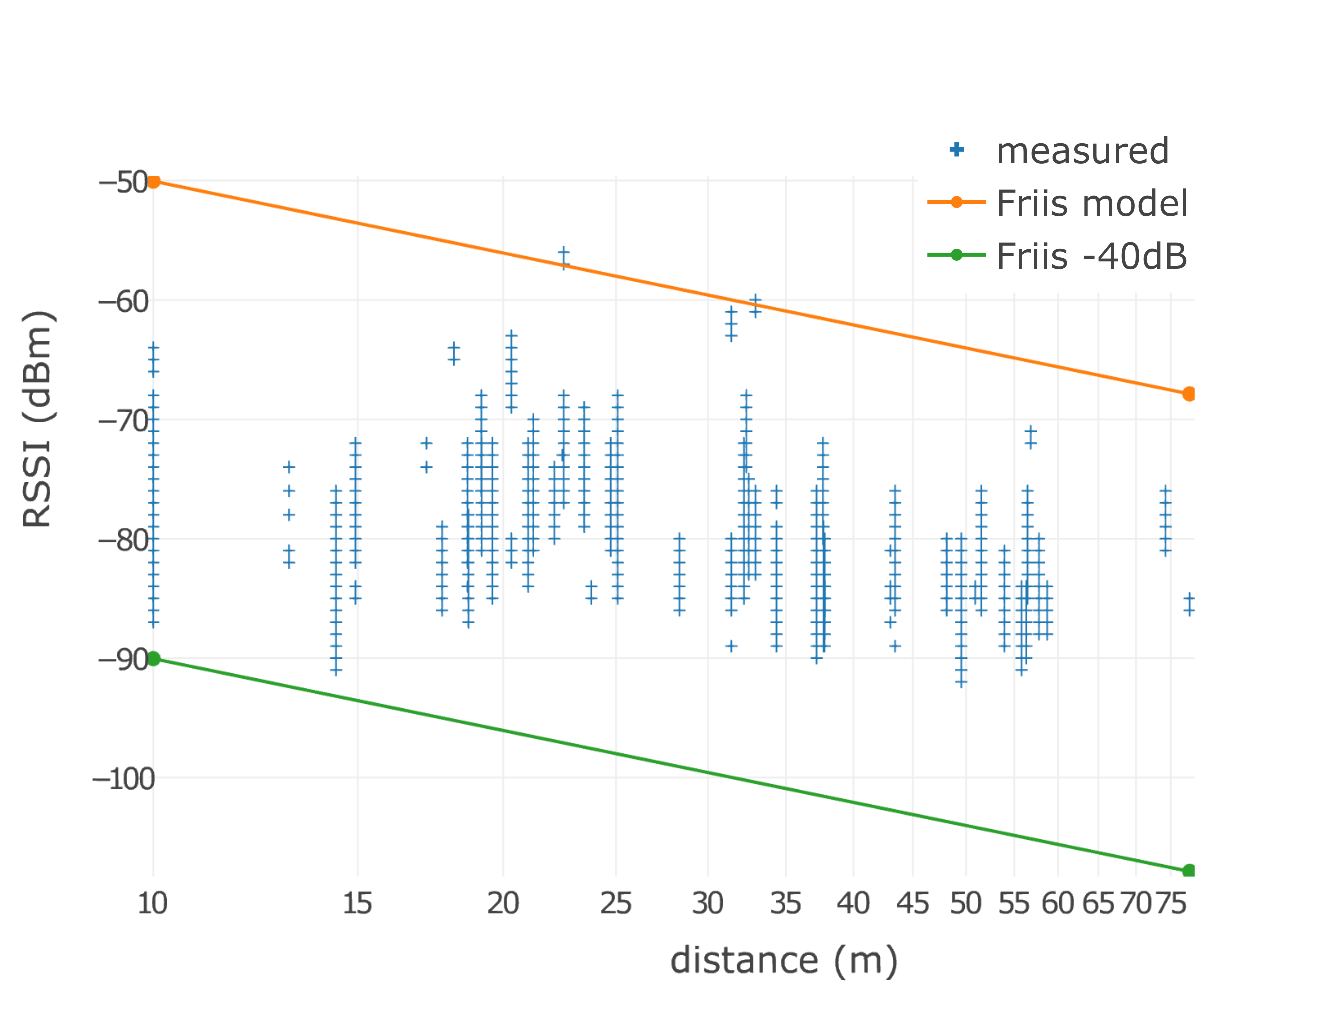
\includegraphics[width=0.5\textwidth]{pister_hack.eps}
    \caption{RSSI measurements are roughly located between the Friis model and the Friis model shifted by $-$40~dB.}
    \label{fig:pister_hack}
\end{figure}

%------------------------------------------------------------------------------
\subsection{Wireless Waterfall}
\label{sec:waterfall}

% sample presentation

Due to the inherent physical unreliability of the radio medium, it is impossible to know if a future transmission will be successful or not.
The Packet Delivery Ratio (PDR) is the portion of successful link-layer transmissions over the total number of link-layer transmission attempts.
A failed attempt means that the link-layer frame needs to be re-transmitted; it does \textit{not} mean the packet is lost.
Over a period of 3~months, \PEACHNUMHRNEIGHBORS~\HRNEIGHBORS messages are collected in the PEACH deployment and \EVANUMHRNEIGHBORS in the EVAlab deployment.
These contain, for a given node, the number of link-layer transmission attempts and successes to each of its neighbors.
We remove the portion of neighbors with no transmission and keep only the DC9003 motes, resulting in a total of 88,284 messages (approx. 37\% from the total number of \HRNEIGHBORS) for the PEACH deployment and a total of 144,187 messages (approx. 32\%) for the EVAlab deployment.

% plot

Fig.~\ref{fig:waterfall} plots the PDR and the RSSI of these 88,284 and 144,187 messages.
For readability, we also plot the average/deviation of the data for a given RSSI value.
Because of its shape, this is known as the ``waterfall plot''.

\begin{figure}
    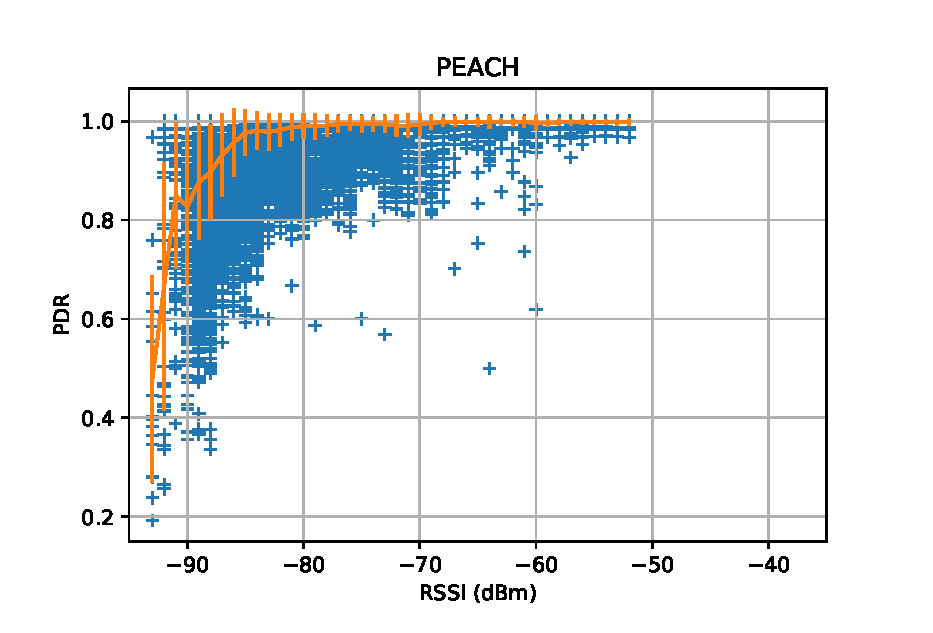
\includegraphics[width=0.5\columnwidth]{waterfall_peach.eps}
    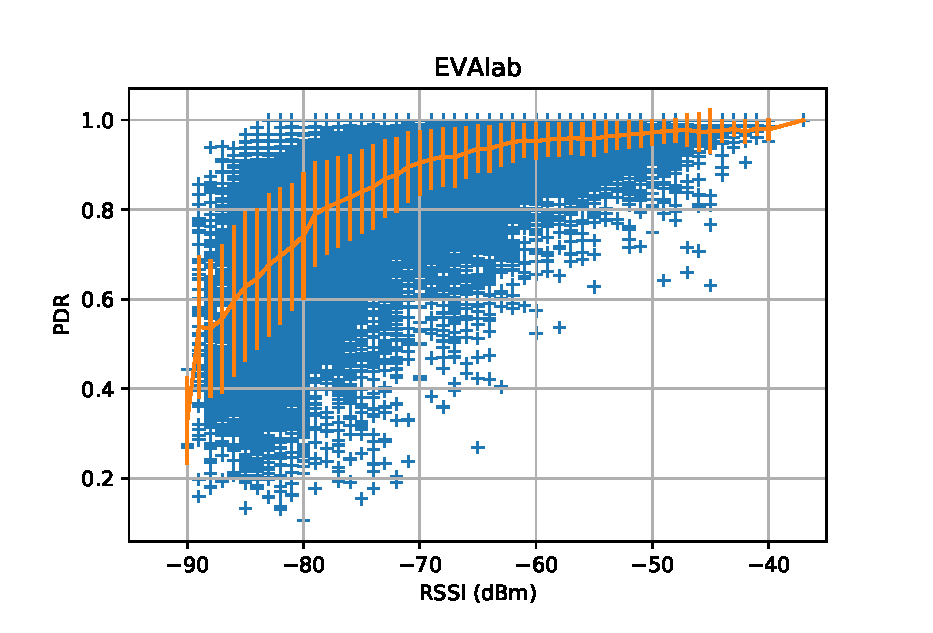
\includegraphics[width=0.5\columnwidth]{waterfall.eps}  
    \caption{
        The PDR/RSSI ``waterfall'' plot. The EVAlab curve is shift right indicating an interference-prone environment.
    }
    \label{fig:waterfall}
\end{figure}

For the PEACH deployment, above $-85~dBm$, the PDR of the link is very good~($>95$\%).
Below that value, the PDR rapidly degrades, indicating that, on these links, frequent retransmissions happen.
For the EVAlab deployment, the PDR starts to degrade at $-60~dBm$.
The device manufacturer documentation~\cite{smip_app_note} indicates that a path is considered as ``bad'' when:

\begin{itemize}
    \item RSSI$>-80~dBm$ and PDR$<50$\%
    \item RSSI$>-70~dBm$ and PDR<70\%
\end{itemize}

This is not the case in any of the two deployments.\\

% interferences

A \textit{waterfall plot} either shifted right with very few paths below $-70~dBm$, or with a non-constantly decreasing curve would be an example of interference-prone environment.
This is not the case for the PEACH deployment, meaning that the \smip network is not experiencing high levels of interferences from co-located wireless devices.
This is the case for the EVAlab deployment, meaning that the \smip network is experiencing external interferences.
Those results correspond to the environment described in Section~\ref{sec:intro}. 

%------------------------------------------------------------------------------
\subsection{End-to-End Reliability}
\label{sec:net_reliability}

% steady state results

We expect the \smip network to offer wire-like reliability.
Table~\ref{tab:net_stats} confirms that this is the case.
It presents statistics gathered over July 15-25 2016 period in the PEACH orchard and from the 2nd of November 2016 to the 16th of February 2017 in the EVAlab	.

\begin{table}
    \begin{tabular}{|l|l|l|}
        \toprule
        {}	 							& PEACH 				  & EVAlab \\
        \midrule
        reliability (Arrived/Lost) 		& 100\% (693,844/0) 	  & 100\% (419,612/0)\\ \hline
        average PDR (Transmit/Fails) 	& 95\% (4,405,569/258778) & 87\% (19,807,535/2,488,149)\\ \hline
        latency     					& 700~msec 				  & Not measured\\
        \bottomrule
    \end{tabular}
    \caption{The overall network performance in the 15-25 July 2016 period.}
    \label{tab:net_stats}
\end{table}

It shows that, as none of the 693,844 packets generated in the network was lost, the end-to-end reliability is 100\%.
The average PDR over all the links is very high (95\%), indicating that the nodes are deployed close enough to one another.
Finally, the average latency over all nodes is 700~ms.
These results are very similar to the very initial results presented in~\cite{watteyne16peach}, indicating no degradation in performance of the \smip network over the 3~month operation.

%------------------------------------------------------------------------------
\subsection{Network Lifetime}
\label{sec:lifetime}

% description

Each device is powered by a pair of Energizer L-91 AA batteries.
These contain a nominal 3134~mAh of charge, or 2821~mAh when accounting for a 10\% decrease due to manufacturing differences.
A \smip node contains a ``charge accounting'' feature in which it tracks the amount of charge is has been drawing from the battery.
Each mote reports this number every 15~min as a field in its \HRDEVICE health report.
This number allows us to predict the lifetime of the device.

% results

Table~\ref{tab:stats_charge} shows charge consumed by the motes over the two 3~month periods, as well as the portion of the battery this represents.
Assuming the same energy consumption rate, we can extrapolate the lifetime.
The node with the longest lifetime is {\tt 60-02-4b}.
From Fig.~\ref{fig:map}, we can see that this is a leaf node.
Since it does not have to relay data from any children, it is normal that this node consumes very little.
The node with the shortest lifetime is {\tt 60-03-82} and has 5~years of lifetime.
This shows the ultra-low power consumption of the \smip network.

\begin{table}
\begin{subtable}{.4\textwidth}
    \begin{tabular}{|c|c|r|}
        \toprule
        MAC    & charge consumed           &   lifetime \\
        \midrule
        \tt{30-60-ef}  & 228~KC (2.2\%) & 11~years \\
        \tt{38-0f-66}  & 252~KC (2.5\%) & 10~years \\
        \tt{3f-f8-20}  & 291~KC (2.9\%) & 8~years \\
        \tt{3f-fe-87}  & 393~KC (3.9\%) & 6~years \\
        \tt{3f-fe-88}  & 458~KC (4.5\%) & 5~years \\
        \tt{58-32-36}  & 328~KC (3.2\%) & 8~years \\
        \tt{60-01-f8}  & 252~KC (2.5\%) & 10~years \\
        \tt{60-02-1b}  & 222~KC (2.2\%) & 10~years \\
        \tt{60-02-4b}  & 146~KC (1.4\%) & 17~years \\
        \tt{60-03-82}  & 495~KC (4.9\%) & 5~years \\
        \tt{60-05-5f}  & 275~KC (2.7\%) & 9~years \\
        \tt{60-05-69}  & 437~KC (4.3\%) & 6~years \\
        \tt{60-05-78}  & 304~KC (3.0\%) & 8~years \\
        \tt{60-05-ab}  & 285~KC (2.8\%) & 9~years \\
        \tt{60-06-27}  & 322~KC (3.2\%) & 8~years \\
        \tt{60-08-d5}  & 263~KC (2.6\%) & 9~years \\
        \bottomrule
    \end{tabular}
    \caption{PEACH}
\end{subtable}\hfill
\begin{subtable}{.45\textwidth}
    \begin{tabular}{|c|c|c|}
        \toprule
        MAC &  charge consumed & lifetime \\
        \midrule
        \tt{38-03-dd} &  566~KC (7.1\%)  &  4 years \\
        \tt{58-e9-ca} &  440~KC (5.6\%)  &  5 years \\
        \tt{58-e9-cb} &  457~KC (5.8\%)  &  5 years \\
        \tt{58-eb-5b} &  472~KC (6.0\%)  &  5 years \\
        \tt{58-eb-64} &  362~KC (4.6\%)  &  6 years \\
        \tt{58-eb-67} &  498~KC (6.3\%)  &  5 years \\
        \tt{58-f3-17} &  384~KC (4.8\%)  &  6 years \\
        \tt{58-f4-f8} &  428~KC (5.4\%)  &  5 years \\
        \tt{58-f5-23} &  464~KC (5.9\%)  &  5 years \\
        \tt{58-f5-3c} &  463~KC (5.8\%)  &  5 years \\
        \tt{58-f5-58} &  429~KC (5.4\%)  &  5 years \\
        \tt{58-f8-8f} &  468~KC (5.9\%)  &  5 years \\
        \tt{58-f9-c4} &  348~KC (4.4\%)  &  7 years \\
        \bottomrule
    \end{tabular}
    \caption{EVAlab}
\end{subtable}\hfill
\caption{Per-node power consumption and associated expected lifetime when powered by a pair of AA batteries.}
\label{tab:stats_charge}
\end{table}
%==============================================================================
\section{Not so Intuitive Results}
\label{sec:notsointuitive}

Results from Section~\ref{sec:intuitive} are ``intuitive'' is that they corroborate previous measurements~\cite{watteyne16peach} or confirm theoretical/lab results~\cite{watteyne10mitigating,watteyne09reliability,watteyne15industrial}.
This section presents results which we believe go against popular belief.
This classification is necessarily subjective.

In Section~\ref{sec:symmetry}, we show that links are, in fact, symmetric.
In Section~\ref{sec:net_stability}, we show that, through the use of TSCH, the low-power wireless topology is, in fact, extremely stable.

%------------------------------------------------------------------------------
\subsection{Link (A)Symmetry}
\label{sec:symmetry}

% what is reported

Motes report the average RSSI value of the packets received from each neighbor in their \HRNEIGHBORS health reports.
Because the network uses channel hopping, these reported RSSI values are also averaged over 15 IEEE802.15.4 frequencies~\cite{std_ieee802154_2011}.
In this section, we use the term ``RSSI'' to denote the average RSSI over 15 frequencies.

% what is asymmetry

A common assumption is that links between neighbor low-power wireless devices are hugely asymmetric.
That is, on a link between nodes $A$ and $B$, $A$ receives $B$'s link-layer frames with an RSSI very different from the frames $B$ receives from $A$.
Numerous routing protocols (often standardized~\cite{rfc3626}) reuse that assumption and start with a costly step of filtering out asymetric links.

% what we measure

We look at the link statistics between the 18th of June 2016 and the 4th of July 2016 (16 days).
The sample contains 411,132 \HRNEIGHBORS messages received from 14 DC9003 nodes (same hardware).
During that period, 21~links are active with at least 250~transmissions for each link.
For each of those links, we compute the difference between average RSSI in each directions.
Results are presented in Fig.~\ref{fig:tab_symmetry}.

\begin{figure}
    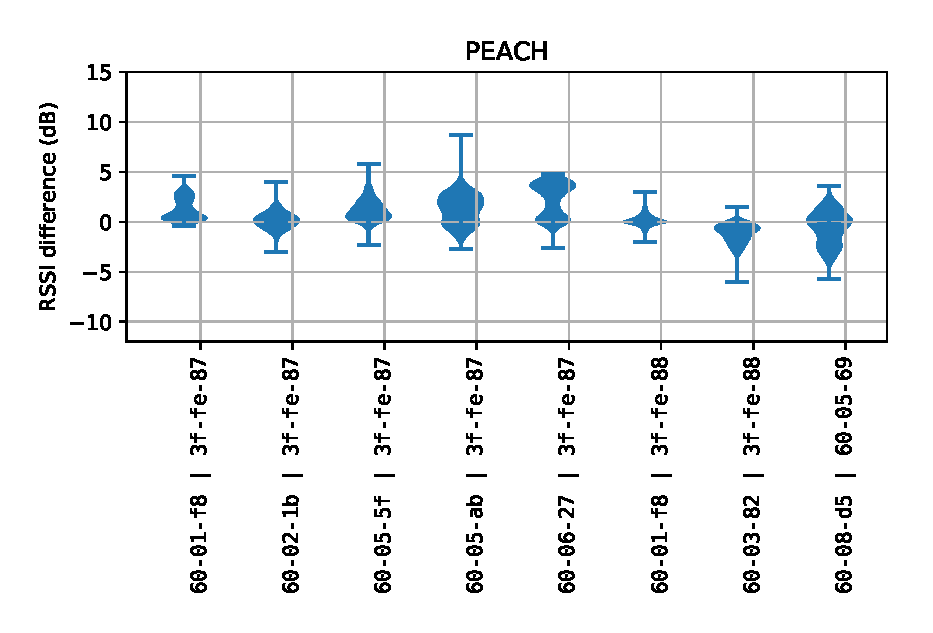
\includegraphics[width=0.5\columnwidth]{asymmetry_peach.eps}
    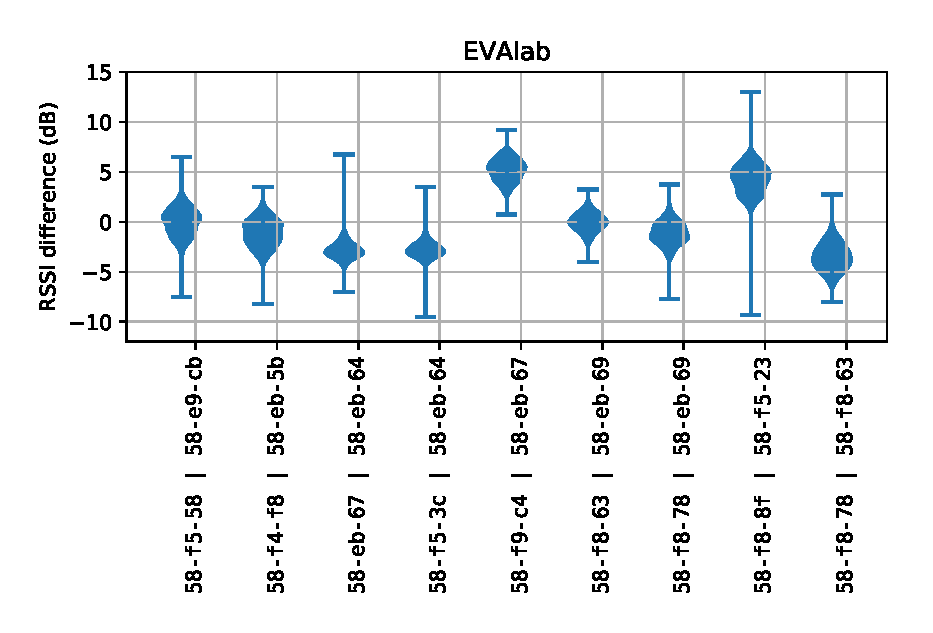
\includegraphics[width=0.5\columnwidth]{asymmetry.eps}
    \caption{
        The difference in RSSI between the two directions of 7/12~wireless links in the PEACH/EVAlab deployment.
        The violin plots show the distribution of the value and the standard deviation.
    }
    \label{fig:tab_symmetry}
\end{figure}

% discussion

Fig.~\ref{fig:tab_symmetry} shows that the RSSI difference never exceeds a couple of dB.
Looking at Fig.~\ref{fig:waterfall}, this translates into a handful of percentage points difference in PDR only.
This means the links can be considered symmetric.
This result is in-line with the physical phenomenon that the signal traveling from $A$ to $B$ undergoes the same attenuation as that from $B$ to $A$.
This result would \textit{not} hold if the neighbor radios had a different transmit power or sensitivity.
That being said, discussions on link symmetry at the routing layer is largely artificial, as any ``good'' medium access control (MAC) protocol uses link-layer acknowledgments.

%------------------------------------------------------------------------------
\subsection{Network Stability}
\label{sec:net_stability}

% unreliability

\lorem

% time scale

\lorem

% dataset

\lorem

% results

\lorem

\begin{figure}
    \includegraphics[width=0.5\columnwidth]{net_churn_peach.eps}
    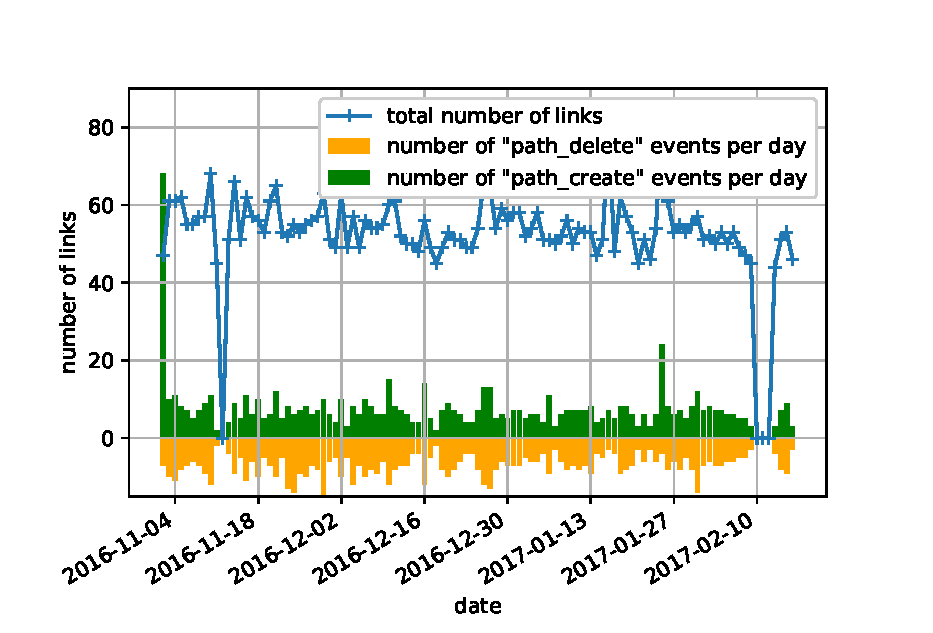
\includegraphics[width=0.5\columnwidth]{net_churn.eps}
    \caption{
        Network stability: the number of \pathcreate and \pathdelete events generated per day over a 16-day period.
        The top portion shows the total number of links.
    }
    \label{fig:net_churn}
\end{figure}

% discussion

\lorem

%==============================================================================
\section{Conclusion}
\label{sec:conclusion}

% intro

\lorem

% intuitive

\lorem

% non-intuitive

\lorem

% conclusion

\lorem

%==============================================================================
%\bibliographystyle{abbrv}
%\bibliography{brun16intuitive}

\begin{thebibliography}{10}

\bibitem{std_ieee802154_2011}
{802.15.4-2011: IEEE Standard for Local and metropolitan area networks. Part
  15.4: Low-Rate Wireless Personal Area Networks (LR-WPANs)}, 5 September 2011.

\bibitem{std_ieee802154e_2012}
{802.15.4e-2012: IEEE Standard for Local and metropolitan area networks--Part
  15.4: Low-Rate Wireless Personal Area Networks (LR-WPANs) Amendment 1: MAC
  sublayer}, 16 April 2012.

\bibitem{rfc3626}
T.~H. Clausen and P.~Jacquet.
\newblock {Optimized Link State Routing Protocol (OLSR)}, October 2003.

\bibitem{smip_app_note}
Linear Technology.
\newblock {\em {SmartMesh IP Application Notes}}, 2015.

\newpage

\bibitem{saunders07antennas}
S.~R. Saunders and A.~Arag\'on-Zavala.
\newblock {\em {Antennas and Propagation for Wireless Communication Systems}}.
\newblock Wiley-Blackwell, 2nd edition, 2007.

\bibitem{srinivasan08beta}
K.~Srinivasan, M.~A. Kazandjieva, S.~Agarwal, and P.~Levis.
\newblock {The $\beta$-factor: Measuring Wireless Link Burstiness}.
\newblock In {\em Conference on Embedded Network Sensor Systems (SenSys)},
  pages 29--42, Raleigh, NC, USA, 2008. ACM.

\bibitem{watteyne16peach}
T.~Watteyne, A.~L. Diedrichs, K.~Brun-Laguna, J.~E. Chaar, D.~Dujovne, J.~C.
  Taffernaberry, and G.~Mercado.
\newblock {PEACH: Predicting Frost Events in Peach Orchards Using IoT
  Technology}.
\newblock {\em {EAI Endorsed Transactions on the Internet of Things}}, June
  2016.

\bibitem{watteyne10mitigating}
T.~Watteyne, S.~Lanzisera, A.~Mehta, and K.~S. Pister.
\newblock {Mitigating Multipath Fading through Channel Hopping in Wireless
  Sensor Networks}.
\newblock In {\em IEEE International Conference on Communications (ICC)}, pages
  1--5, Cape Town, South Africa, 23-27 May 2010. IEEE.

\bibitem{watteyne09reliability}
T.~Watteyne, A.~Mehta, and K.~Pister.
\newblock {Reliability Through Frequency Diversity: Why Channel Hopping Makes
  Sense}.
\newblock In {\em International Symposium on Performance Evaluation of Wireless
  Ad Hoc, Sensor, and Ubiquitous Networks (PE-WASUN)}, pages 116--123,
  Tenerife, Canary Islands, Spain, 26-30 October 2009. ACM.

\bibitem{watteyne15industrial}
T.~Watteyne, J.~Weiss, L.~Doherty, and J.~Simon.
\newblock {Industrial IEEE802.15.4e Networks: Performance and Trade-offs}.
\newblock In {\em International Conference on Communications (ICC), Internet of
  Things Symposium}, London, UK, 8-12 June 2015. IEEE.

\bibitem{zats10wireless}
S.~Zats.
\newblock {Wireless Sensor Networks Scaling and Deployment in Industrial
  Automation}.
\newblock Master's thesis, University of California, Berkeley, 13 May 2010.

\end{thebibliography}

\end{document}
